\section{Einleitung}
\label{s:intro}


%%%%%%%%%%%%%%%%%%%%%%%%%%%%%%%%%%%%%%%%%%%%%%%%%%%%%%%%%%%%%%
\subsection{Ein Abschnitt der Einleitung}
\label{ss:intro:abc}

Einen Überblick findet man z.\,B.\ in \cite{Auer00:HTF}.

\begin{figure}[t]
\centering

\begin{subfigure}{0.45\linewidth}
\centering
%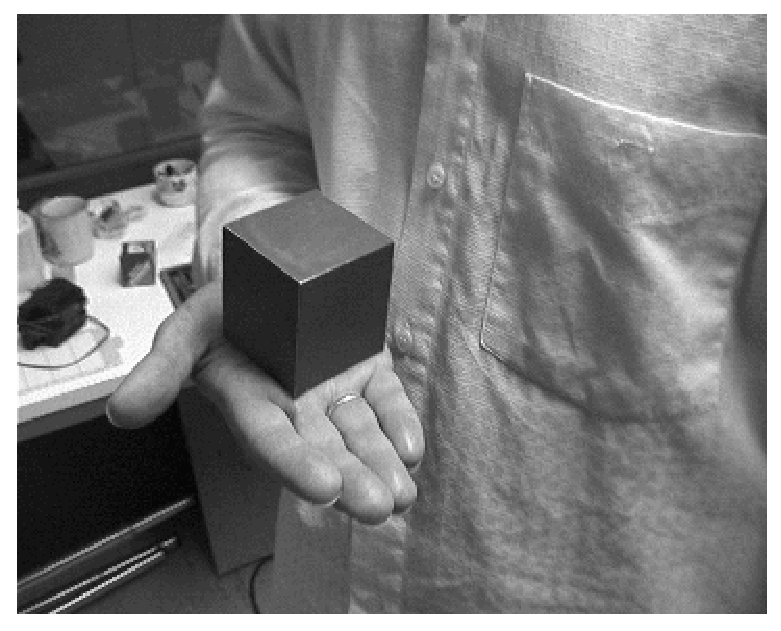
\includegraphics[width=\linewidth]{\figdir/handorig}
\caption{Originalbild}
\label{FIG:arexorig}
\end{subfigure}
%
\begin{subfigure}{0.45\linewidth}
\centering
%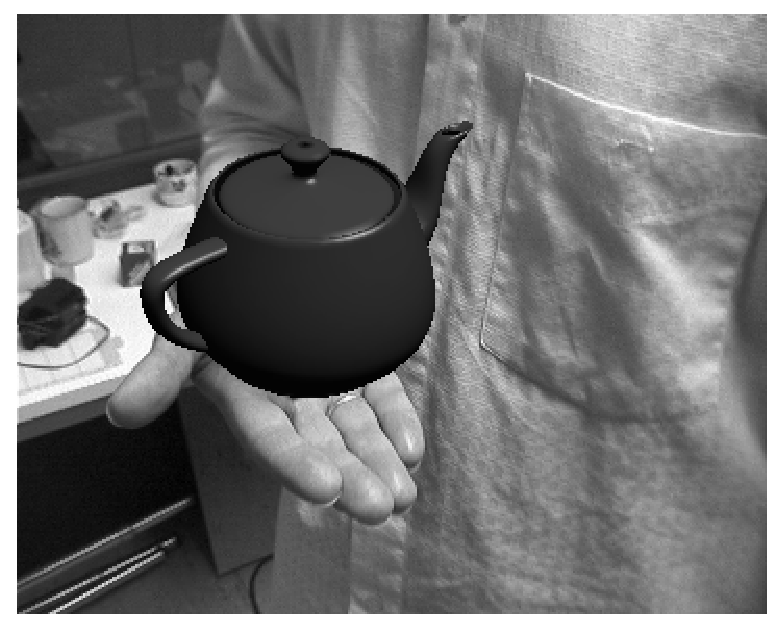
\includegraphics[width=\linewidth]{\figdir/handaug}
\caption{erweitertes Bild}
\label{FIG:arexaugm}
\end{subfigure}
%
\caption[AR Beispiel]
{Beispiel eines Augmented Reality Systems: es folgt eine Beschreibung (Bilder aus \cite{Schmidt01:PAO})}
\label{FIG:arex}
\end{figure}

Ein Beispiel wird in Abb.\ \ref{FIG:arex} gezeigt.
Das verwendete Objekt ist in Abb.\ \ref{FIG:arexorig} dargestellt, das Ergebnis in Abb.\ \ref{FIG:arexaugm}.

Eine Formel
\begin{equation}
\label{eq:cvp:test}
f(x) = \frac{1}{3} x + 5, \quad x \in \real.
\end{equation}

Und noch eine:
\begin{equation}
\label{eq:cvp:matvec}
\bm{M}  = \bm{Ax} \pi, \quad \bm{A} \in \real^{2 \times 2}, \bm{x} \in \real^2.
\end{equation}

Tabelle \ref{t:CodebookOverview} gibt einen Überblick über XYZ.

\begin{table}[t]
\centering\small
%
% generated by TexTableGenerator.pl ((c) Florian Vogt)
% from file: /home/Jochen/data/dissdata/results/CodebookOverview.log
%
\begin{tabular}{l|ccc|cc}
\hline
\hline
                  \textbf{Sequence} &          ARTS &           wman &         stcams &         ARTVZ &        ARTSUZ \\ 
                 \textbf{\# Frames} &             190 &              40 &             400 &             270 &             190 \\ 
     \textbf{\# relative movements} &           17955 &             780 &           79800 &           36315 &           17955 \\ 
\textbf{\# movements after pre-sel.} &           14336 &             623 &           37915 &           21788 &           14343 \\ 
       \textbf{min.\ angle in seq.} &   0.233$^\circ$ &    5.95$^\circ$ &   0.154$^\circ$ & 0.00000171$^\circ$ &  0.0388$^\circ$ \\ 
       \textbf{max.\ angle in seq.} &    81.7$^\circ$ &     180$^\circ$ &    47.3$^\circ$ &    80.3$^\circ$ &    80.9$^\circ$ \\ 
\textbf{min.\ angle after pre-sel.} &    12.9$^\circ$ &    21.1$^\circ$ &    17.3$^\circ$ &    16.3$^\circ$ &    12.9$^\circ$ \\ 
\textbf{max.\ angle after pre-sel.} &    81.7$^\circ$ &     161$^\circ$ &    47.3$^\circ$ &    80.3$^\circ$ &    80.9$^\circ$ \\ \hline\hline
\end{tabular}

 \caption[Testtabelle]{Datenselektion für verschiedene Testdatensätze.}
  \label{t:CodebookOverview}
\end{table}

\section{Technische Grundlagen und Implementierungen}
\label{s:grundlagen}

Im folgenden Kapitel wird ein Überblick über die zentralsten \ac{ble} Anwendungen gegeben. Zusätzlich wird die Hardwareebene im Bezug auf die physikalischen Voraussetzungen und die genutzten Frequenzbereiche näher betrachtet. 

\subsection{Beispiele für Implementierungen}
\label{ss:grundlagen:beispiele}

Im einundzwanzigsten Jahrhundert steigt die Verwendung von Geräten, welche drahtlos mit einem Empfangsgerät kommunizieren können. Vor allem die Einführung des Smartphones hat an diesem Punkt die drahtlose Kommunikation vorangetrieben. Nutzer wollen viele Funktionen zur Verfügung gestellt bekommen, um den persönlichen Alltag einfacher gestalten zu können.\\

\noindent Schon vor der Einführung des Smartphones war das Kommunikationsprotokoll "`Bluetooth"' auf Mobiltelefonen verfügbar. Dabei wurde es hauptsächlich zum Datentransfer zwischen zwei Bluetoothfähigen Endgeräten verwendet. Das Hauptproblem, welches der Nutzer dabei erfahren musste, ist, dass diese Form der Datenübertragung sehr viel Zeit in Anspruch genommen hat. Dies lässt sich auf die geringe Datenmenge zurückführen, die pro Paket möglich ist.\\

\noindent Nachdem das Smartphone immer mehr an Beliebtheit gewonnen hat und sich der Begriff des \ac{iot} entwickelt hat, reagierte die Bluetooth \ac{sig}, indem sie ein Protokoll erarbeiteten, welches einen möglichst geringen Stromverbrauch, eine geringe Bandbreite und niedrige Komplexität bietet \cite{Townsend14:GSB}.\\

\noindent Mit der Einführung von \ac{ble} kam die Möglichkeit kleine Datensignale zwischen Geräten auszutauschen. Ein aktuell sehr bekanntes Beispiel sind dabei sogenannte "`Smartwatches"'. Diese bieten neben der Möglichkeit die Uhrzeit bereitzustellen viele weitere Funktionen, wie beispielsweise die Steuerung von Telefongesprächen, oder die Fernsteuerung der Musikwiedergabe. Der Nutzer erhält durch ein derartiges Gerät die Möglichkeit, sein Smartphone in gewissen Bereichen fernzusteuern.\\

\noindent Beinahe jeder Mensch in der heutigen Zeit besitzt und nutzt ein Smartphone. Jedes Smartphone ist dabei mit einer Bluetoothschnittstelle ausgestattet. Dieser Sachverhalt liefert die Möglichkeit, nicht nur eine "`Smartwatch"' mit dem Smartphone zu verbinden, sondern jegliches Empfangsgerät, welches der Nutzer benötigen könnte. Besonders beliebt sind dabei Fitnessgeräte, die dem Nutzer Informationen über sein Fitnesslevel liefern.\\

\noindent Allerdings liefert der Sachverhalt, dass beinahe jeder Nutzer Bluetooth nutzt auch andere "`Usecases"'. Mit sogenannten "`Bluetooth beacons"' (siehe Kapitel \ref{s:ibeacon}) kann man beispielsweise mittels Triangluation die Position einer Person in einem Raum bestimmen. Dies kann beispielsweise bei der Umsetzung von autonomen Supermärkten behilflich sein, um zu bestimmen, welche Lebensmittel der Kunde besucht hat. Auch für die Marktforschung kann dies sehr interessant sein.\\

\noindent Sollte man die Absicht haben, ein eigenes Gerät zu entwickeln, welches mittels \ac{ble} kommuniziert, gibt es mehrere Anbieter für Hardwarekomponenten für verschiedene Anwendungsfälle. Besonders nennenswert sind dabei die Firmen "`Nordic"' und "`Texas Instruments"'.\\

\noindent  

\subsection{Hardware}
\label{ss:grundlagen:hardware}



\subsection{Frequenzbereich}
\label{ss:grundlagen:frequenz}

\section{Funktionsweise Bluetooth Low Energy}
\label{s:funktionsweise}

%%%%%%%%%%%%%%%%%%%%%%%%%%%%%%%%%%%%%%%%%%%%%%%%%%%%%%%%%%%%%%
\subsection{Protokollstack}
\label{ss:funktionsweise:protokollstack}

\subsubsection{Physical Layer}
\label{sss:funktionsweise:physical}

\subsubsection{Linked Layer}
\label{sss:funktionsweise:linked}

\subsubsection{Profile}
\label{sss:funktionsweise:profiles}

\subsection{Kommunikation}
\label{ss:funktionsweise:kommunkation}

\subsubsection{Advertisement}
\label{sss:funktionsweise:advertisement}

\subsubsection{Verbindung}
\label{sss:funktionsweise:verbindung}

\subsubsection{Datenaustausch}
\label{sss:funktionsweise:datenaustausch}

\subsection{Featureset (Kosten, Reichweite, Energieverbrauch, etc... am Titel muss ich noch schrauben)}
\label{ss:funktionsweise:Featureset}

\section{Anwendungsbeispiel iBeacon}
\label{s:ibeacon}

\subsection{Funktionsweise}
\label{ss:ibeacon:funktionsweise}

\subsection{Kommunikation}
\label{ss:ibeacon:kommunikation}

\section{Vergleich mit anderen Kommunikationsprotokollen}
\label{s:vergleich}

\subsection{ZigBee}
\label{ss:vergleich:zigbee}

\section{Fazit}
\label{s:fazit}
%%% Local Variables: 
%%% mode: latex
%%% TeX-master: "thesis.tex"
%%% End: 
